
\documentclass[12pt]{article}

\usepackage{co342}

\begin{document}
\begin{titlepage}
  \centering
  \vspace*{2in}
  {\huge CO342 - Introduction to Graph Theory}\par
  \vspace{0.5in}
  {\large University of Waterloo}\par
  {\large Nicholas Pun}\par
  {\large Fall 2017 (Revised 2021)}\par 
\end{titlepage}

\tableofcontents
\clearpage

\section*{Preface}
\addcontentsline{toc}{section}{Preface}
\section{Connectivity}
\section{Vector Spaces for Graphs}
\section{Planarity}
\section{Matchings}


\begin{minipage}{\textwidth}
  \centering
  \begin{tikzpicture}[scale = 0.75]
      \node[vertex][label=left:{$-10$}] (a) at (0,0) {a};
      \node[vertex][label={$-5$}] (b) at (4.5,3) {b};
      \node[vertex][label=below:{$12$}] (c) at (4.5,-3) {c};
      \node[vertex][label=right:{$3$}] (d) at (9,0) {d};
      
      \begin{scope}[every node/.style={fill = white, ellipse}]
          \draw[directed] (a) to node {$(50,7)$} (b);
          \draw[directed] (a) to node {$(70,5)$} (c);
          \draw[directed] (b) to node {$(20,2)$} (d);
          \draw[directed] (b) to node {$(30,12)$} (c);
          \draw[directed] (c) to node {$(100,8)$} (d);
      \end{scope}
  \end{tikzpicture}
\end{minipage}

\begin{minipage}{\textwidth}
  \centering
  \begin{tikzpicture}[scale = 0.75]
      \node[vertex] (a) at (0,0) {a};
      \node[vertex] (b) at (4.5,3) {b};
      \node[vertex] (c) at (4.5,-3) {c};
      \node[vertex] (d) at (9,0) {d};
      
      \draw[edge] (a) -- (b) -- (d);
      \draw[edge] (a) -- (c) -- (d);
      \draw[path] (b) -- (c);

      \node[box][fit=(a) (b)] {};
  \end{tikzpicture}
\end{minipage}

% \subfile{sections/graph-theory-primer}\clearpage
% \subfile{sections/transshipment-problem/transshipment-problem}\clearpage
% \subfile{sections/min-cost-flow-problem/min-cost-flow-problem}\clearpage
% \subfile{sections/applications-tp-mcfp/applications-tp-mcfp}\clearpage
% \subfile{sections/shortest-dipaths/shortest-dipaths}\clearpage
% \subfile{sections/maximum-flow/maximum-flow}\clearpage
% \subfile{sections/global-min-cut/global-min-cut}\clearpage

\end{document}

% \documentclass[12pt]{article}

% \usepackage[utf8]{inputenc}
% \usepackage[english]{babel}
% \usepackage[margin=1in]{geometry}
% \usepackage{graphicx}
% \usepackage{pdfpages}
% \usepackage{hyperref}
% \usepackage{bookmark}

% \begin{document}

% \begin{titlepage}
%   \centering
%   \vspace*{2in}
%   {\Large (Notes Scans)}\par
%   \vspace{0.3in}
%   {\large University of Waterloo}\par
%   {\large Nicholas Pun}\par
%   {\large Fall 2017}\par 
% \end{titlepage}
 
% \tableofcontents
% \clearpage

% 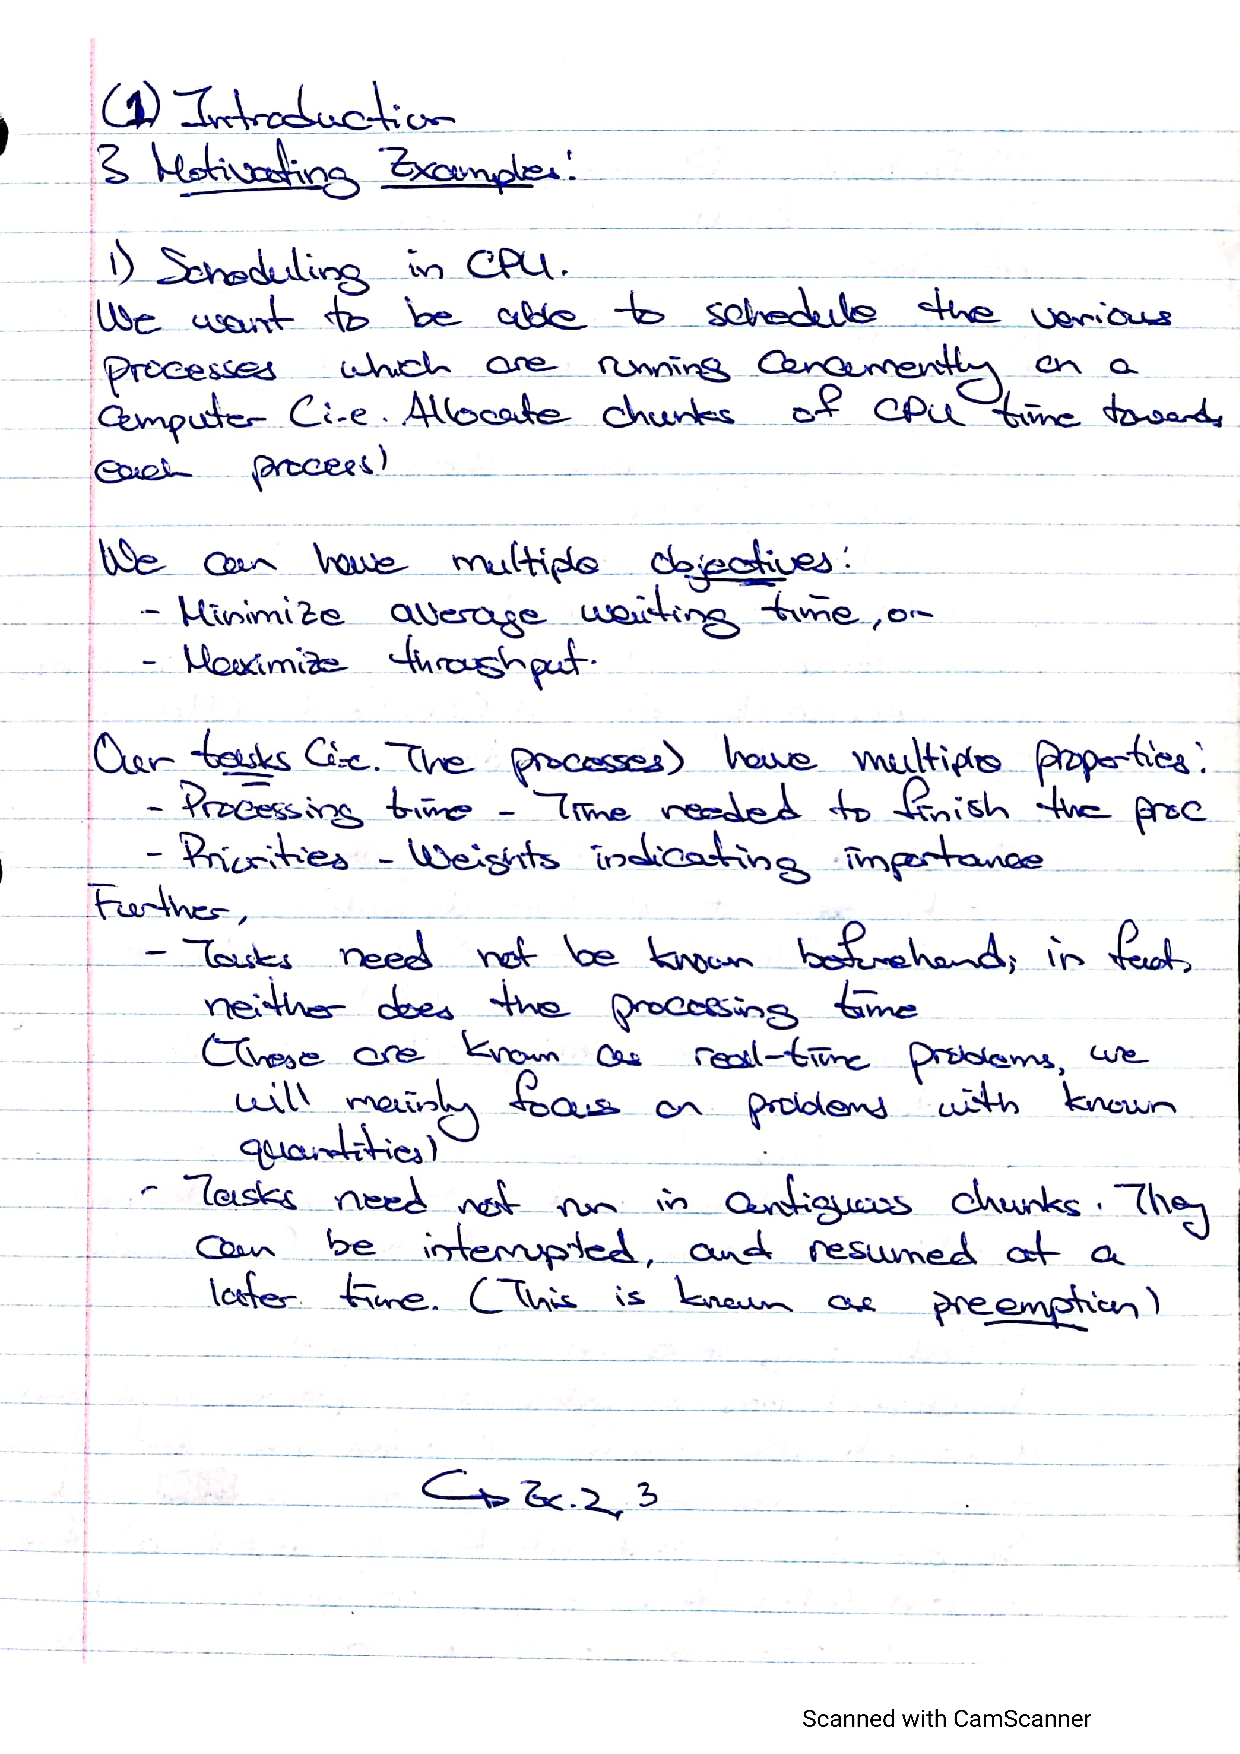
\includepdf[pages=1, pagecommand={\thispagestyle{plain}\section{Connectivity}}]{sections/sec1.pdf}
% \includepdf[pages=2-, pagecommand=\thispagestyle{plain}]{sections/sec1.pdf}
% \clearpage

% 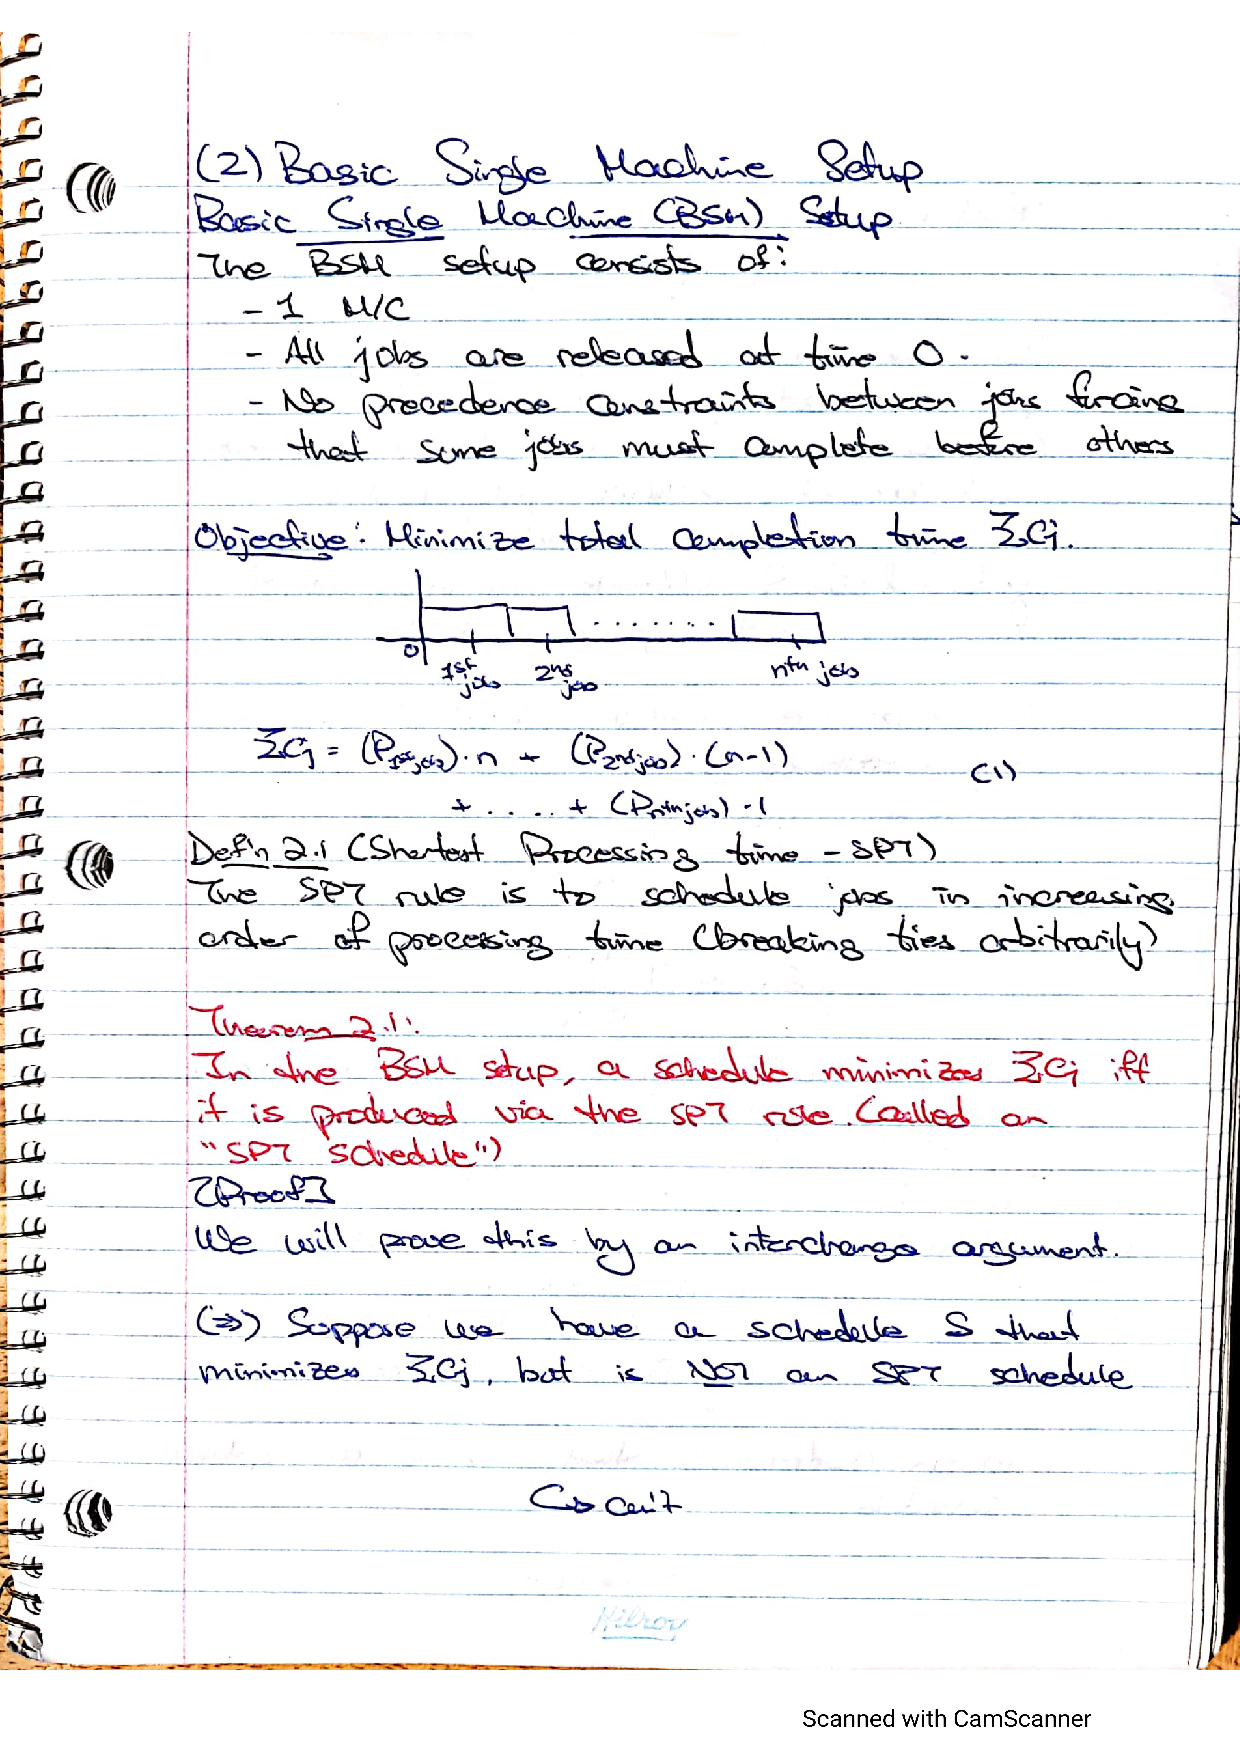
\includepdf[pages=1, pagecommand={\thispagestyle{plain}\section{Vector Spaces for Graphs}}]{sections/sec2.pdf}
% \includepdf[pages=2-, pagecommand=\thispagestyle{plain}]{sections/sec2.pdf}
% \clearpage

% 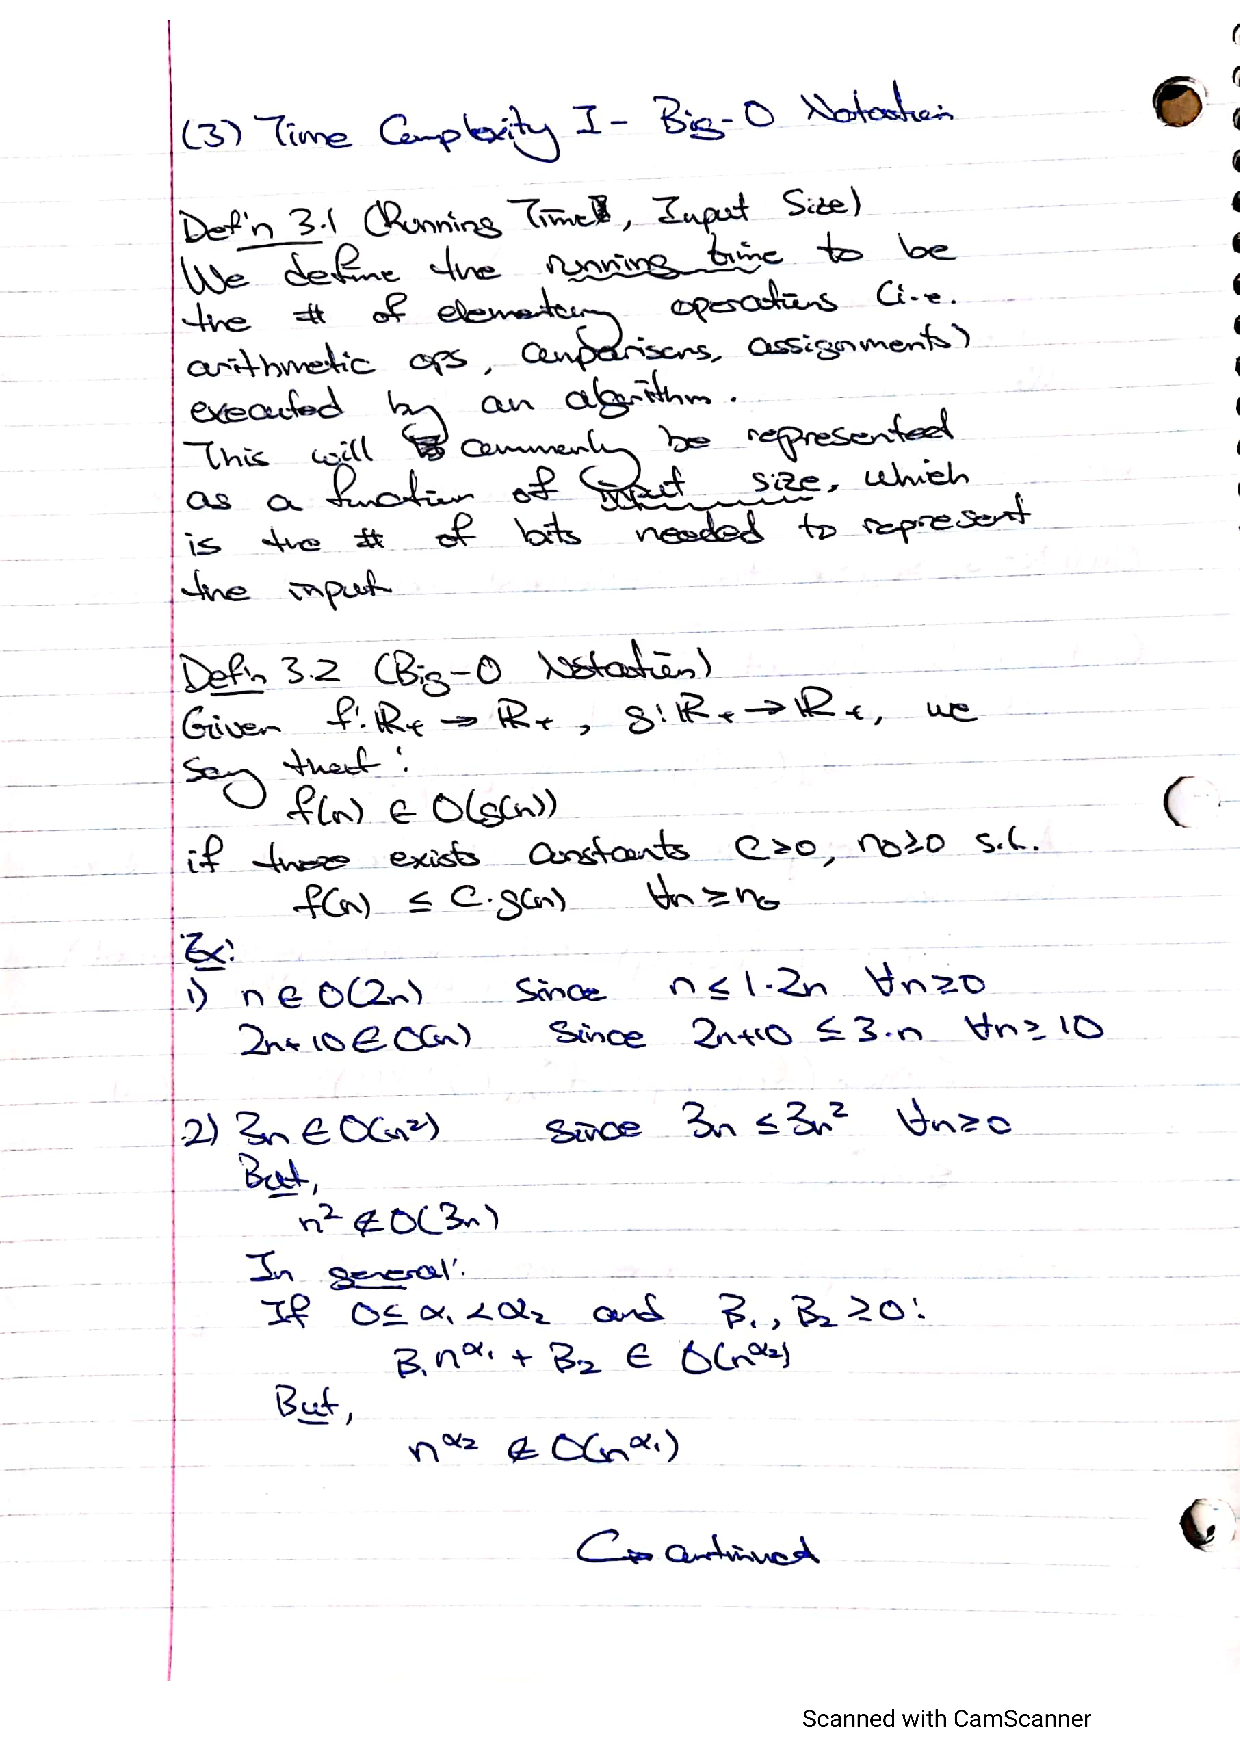
\includepdf[pages=1, pagecommand={\thispagestyle{plain}\section{Planarity}}]{sections/sec3.pdf}
% \includepdf[pages=2-, pagecommand=\thispagestyle{plain}]{sections/sec3.pdf}
% \clearpage

% \includepdf[pages=1, pagecommand={\thispagestyle{plain}\section{Matchings}}]{sections/sec4.pdf}
% \includepdf[pages=2-, pagecommand=\thispagestyle{plain}]{sections/sec4.pdf}
% \clearpage

% \end{document}